% Chapter 2

\chapter{Background on Substation Automation} % Main chapter title

\label{chap:Chapter2} % For referencing the chapter elsewhere, use \ref{chap:Chapter2} 

%----------------------------------------------------------------------------------------
\section{Introduction to Substation Automation System}
In the past, electrical grids faced serious limitations in terms of the employed technologies. However, in today's world, there is a notable increase and significant growth in digital communication technologies in terms of performance and reliability. To adapt to this evolution, Substation Automation Systems (SAS) are based on dedicated software embedded in hardware components. Additionally, SAS provides a straightforward way to control and monitor all equipment in the substation, both locally and remotely. SCADA systems offer users a Human-Machine Interface (HMI) used to control, monitor, and protect devices. Moreover, SAS perform this control and monitoring in real-time, contributing to maximizing availability, efficiency, safety, and data integration, resulting in a significant cost reduction.

Furthermore, the IEC 61850 standard and its associated communication protocols are introduced, to be employed within individual substations and between substations. Consequently, the implementation of the Manufacturing Message Specification (MMS), GOOSE, and SV protocols allows for efficient control and monitoring, ensuring that the system is made more robust and future-proof.

Figure~\ref{fig:substation-automation} is a diagram illustrating how is inside a SAS system, this figure  represents the minimum equipment it is needed to have a substation, as IED, Global Positioning System (GPS), switches, routers, personal computer and all the electrical equipment to manage the grid.\footnote{\url{https://docplayer.net/40767859-Lecture-5-substation-automation-systems-course-map.html}}

\begin{figure}[tbh]
	\centering
	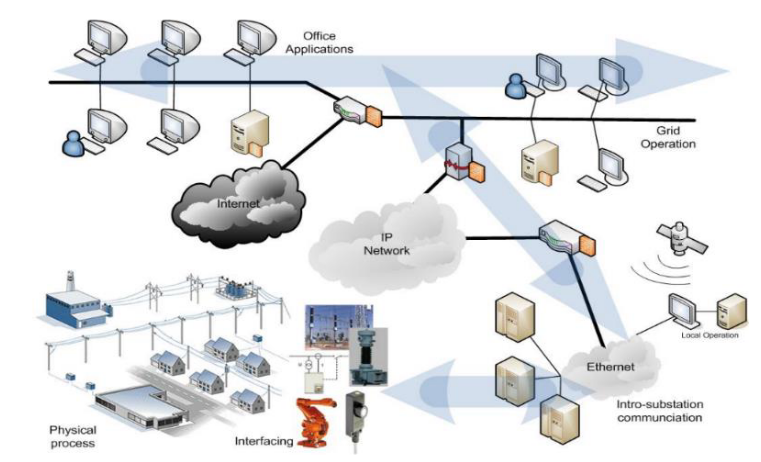
\includegraphics[width=0.8\textwidth, keepaspectratio]{ch2/assets/SAS.png}
	\caption{Design of Substation Automation Systems(Image credits: KTH, "Lecture 5: Substation Automation Systems")}
	\label{fig:substation-automation}
\end{figure}
\FloatBarrier

\section{Backyard System}
The backyard system serves as the hub for all high-power apparatus, responsible for channeling energy from the power plant and facilitating its delivery to homes. It encompasses a range of critical devices, such as high-voltage circuit breakers, switches, voltage transformers for protection and measurement, current transformers for protection and measurement, high-voltage power transformers, capacitor banks, reactors, and synchronous compensators, devices that have gained increasing prominence in recent times. However, let's delve into the components found in any substation, as they will be detailed in the subsequent subsections.

\subsection{Circuit Breakers}
High-voltage circuit breakers play a crucial role in the operation and protection of electrical networks at very high, high, and medium voltages. They are electromechanical devices designed to interrupt the flow of electric current under abnormal conditions in the electrical network, such as short circuits and overloads. In the event of a network fault, the circuit breaker receives a signal from the electrical protection system detecting abnormalities. With this signal, the circuit breaker contacts quickly open to interrupt the electric current and extinguish the electrical arc generated when the contacts open, preventing damage to the network equipment.

Circuit breakers ensure the reliability of electrical power supply, with a focus on making electricity available to the entire network. High-voltage and very high-voltage circuit breakers are responsible for isolating detected faults in the system, preventing the spread of the defect to other parts of the network and thus avoiding widespread blackouts.

\subsection{Switches}
High-voltage switches play a pivotal role in the seamless operation of electrical networks at very high, high, and medium voltages. These electromechanical devices are intricately designed to isolate a section of the electrical system during normal operating conditions. When conducting maintenance on the electrical network, the switch opens a specific circuit segment, necessary for the safe and efficient execution of maintenance tasks. This ensures the well-being of maintenance personnel while simultaneously preserving the continuous operation of the electrical network.

In essence, very high, high, and medium voltage switches serve as integral components in power substations, offering a secure and dependable method for isolating designated sections of the electrical system. This isolation is essential for the maintenance of power system equipment, including transformers, circuit breakers, and capacitor banks. Importantly, this isolation process does not compromise the overall functionality of the substation(~\cite{janne2013switchgear}).

\subsection{Voltage Transformers}
Voltage transformers play a critical role in electrical systems by providing precise voltage measurements for each phase of the circuit. Their primary function is to convert very high voltages into more manageable, general-purpose voltages like 110V. The utilization of lower voltages facilitates easier handling, both in terms of magnitude and the insulation required for compatibility with IEDs.

Ensuring optimal signal quality is a key responsibility of voltage transformers. Their primary objective is to accurately replicate the high voltage in a lower voltage format, creating a precise replica with reduced values. This replication process is essential for utilizing the information in electrical protection, enabling the analysis of network disturbances, and facilitating timely action in the event of a fault.


\subsection{Current Transformers}
Current transformers play a crucial role in electrical systems, offering precise current measurements for each phase of the circuit. Their primary function is to convert very high currents into more manageable, general-purpose currents, typically around 1A. This reduction in current values enhances ease of handling, both in terms of magnitude and the insulation required for compatibility with IEDs.

Ensuring optimal signal quality is a paramount responsibility of current transformers. Their principal objective is to accurately replicate the high current in a lower current format, creating a precise duplicate with reduced values. This replication process is vital for utilizing information in electrical protection, enabling the analysis of network disturbances, and facilitating prompt action in the event of a fault.

\section{Intelligent Electronic Devices}
The IED formed by the set of units for data acquisition, processing, and transmission, located in substations, is generically referred to as a Remote Terminal Unit (RTU). At a given moment, it represented a significant evolution within a sector known for its conservatism in adopting new technologies, allowing remote control of substations by a central-level system, initiating the evolution of data transmission capacity through advances in telecommunications and the application of computers on a large scale. This enabled the expansion of the potential use of digital technology as a reality in substation environments(~\cite{NormaIEC61850}).

With consolidated digital electronics technology, the first proposals for Integrated Protection and Control Systems emerged, using protection relays and control units based on microprocessors and memories, with intelligence at the equipment level for logic execution and automation, introducing the concept of IED. These devices enable the use of computer networks for communication via fiber optics between terminals and relays within the same substation. In addition, personal computers are used at the control and monitoring level of the substation (~\cite{NormaIEC61850}).

\subsection{Protection Alghorithm System}
Protection stands as one of the paramount functions within a substation or any power system. Its primary goal is to ensure the safeguarding of equipment and personnel, while also minimizing damage in the event of electrical faults, short circuits, or overloads. This critical function is inherently local, designed to operate independently if necessary, irrespective of the substation's automation system. Even though it seamlessly integrates into the automation system under normal conditions, the integrity and effectiveness of protection functions should never be compromised or restricted within any power system automation (~\cite{NormaIEC61850}).

\subsection{Control System}
Local control involves autonomous control actions that a device can independently perform, such as interlocks, switching sequences, synchronism verification, and others. In this context, human intervention is limited, and the risks of errors are minimized. Similar to protection, local control should continue to operate even if the automation system is compromised.

Remote control functions are related to substation control executed by SCADA software. Commands can be directly issued to devices managed remotely, such as opening or closing a circuit breaker. Relay settings can be adjusted either through the device itself or a computer equipped with manufacturer-specific software. Additionally, desired information can be collected from protection relays using the IEC~61850 protocol via the MMS protocol. This eliminates the need for human actions within the substation to perform switching operations, making these actions faster. Furthermore, the SCADA terminal provides an overview of the entire plant, offering insights into ongoing activities and status (~\cite{NormaIEC61850}).

\subsection{Measurement}

A range of information from a substation is collected and analyzed in real-time by the automation system for its proper functioning. The measurement system consists of:

\begin{itemize}
	\item Electrical Measurements - voltages, currents, power, power factor, harmonics, etc;
	\item Monitoring Measurements of Equipment - such as transformer and motor temperatures;
	\item Disturbance Recorder - Recordings of disturbances for fault analysis.
\end{itemize}

This vast amount of information can assist in studies such as load flow analysis and planning for disturbances, in addition to being essential for protection and control functions (~\cite{NormaIEC61850}).

\subsection{Monitoring}
It is a sequence of events or part of the automation system with information that allows monitoring the state of the substation, such as equipment status, maintenance alerts, relay configurations, etc. This improves the overall system efficiency, enhancing the effectiveness of protection and control. These pieces of information are useful in fault analysis, determining what happened, when, where, and how it happened (location, time, and sequence)(~\cite{NormaIEC61850}).

\subsection{Communication Protocols}
The significant progress in substation automation has led to substantial investments by major IED manufacturers aiming to provide differentiation in protection and control equipment for substations. This competition has also given rise to a large number of proprietary communication protocols, which, to some extent, generated undesirable results in terms of interoperability. Substations with a large number of IEDs are highly likely to have undergone growth, with the current topology not being the original one. In such cases, equipment from different manufacturers is often present, and when connected to a single network, they do not communicate as expected in the vast majority of cases.

Faced with the communication challenges between devices, standardized protocols have emerged with the goal of achieving the desired interoperability. In other words, these protocols aim to enable communication between devices from different manufacturers on the same network. Figure~\ref{fig:table-protocols} displays some of the most commonly used protocols in substation networks (~\cite{NormaIEC61850}).

\begin{table}[h]
	\centering
	\scriptsize
	\resizebox{\textwidth}{!}{
		\begin{tabular}{@{}lcccc@{}}
			\toprule
			\textbf{Protocol} & \textbf{Originally used by} & \textbf{Speed} & \textbf{Access Principle} & \textbf{OSI Layers} \\ \midrule
			MODBUS                      & Gould-Modicon                    & 19.2 kbps           & Cyclic scanning             & 1, 2, 7              \\
			SPABUS                      & ABB (exclusive)                  & 19.2 kbps           & Cyclic scanning             & 1, 2, 7              \\
			DNP3.0                      & GE-Harris                        & 19.2 kbps           & Cyclic scanning\textsuperscript{2}            & 1, 2, 7\textsuperscript{3}             \\
			IEC 60870-5                 & All manufacturers                & 19.2 kbps           & Cyclic scanning             & 1, 2, 7              \\
			MODBUS+                     & Gould-Modicon                    & Token               & Cyclic scanning             & 1, 2, 7              \\
			PROFIBUS                    & Siemens                          & 12 Mbps             & Token                        & 1, 2, 7              \\
			MVB                         & ABB                              & 1.5 Mbps            & TDM                          & 1, 2, 7\textsuperscript{4}             \\
			FIP                         & Merlin-Gerin                     & 2.5 Mbps            & TDM                          & 1, 2, 7              \\
			Ethernet + TCP/IP           & All manufacturers                & 10 Mbps             & CSMA/CD                      & 1-7                  \\
			LON                         & ABB (exclusive)                  & 1.25 Mbps           & PCMSA/CD                     & 1-7                  \\
			UCA 2.0                     & GE                               & 10 Mbps             & CSMA/CD                      & 1-7                  \\ \bottomrule
		\end{tabular}
	}
	\caption{Communication Protocols used by energy company.}
	\label{table:protocols}
\end{table}



\section{Overview of IEC~61850}
IEC 61850 is an international standard for communication in substations and power utility automation. It defines a set of protocols and data models to enable the interoperability of devices within a substation, facilitating efficient and standardized communication for protection, control, monitoring, and automation purposes. Key features of IEC 61850 include:

\begin{itemize}
	\item Data Modeling: The standard introduces a standardized way of modeling substation data, using a hierarchical structure known as the Common Information Model (CIM). This allows for consistent representation of information across different devices.
	\item Communication Protocols: IEC 61850 specifies communication protocols for substation automation, with an emphasis on Ethernet-based communication. It defines how devices such as protection relays, controllers, and meters exchange information using protocols like MMS and GOOSE.
	\item Sampled Values: Part 9 of the standard, IEC 61850-9, introduces Sampled Values, enabling the transmission of digitized analog values, such as voltages and currents, in a standardized manner. This is crucial for real-time protection applications.
	\item Configuration Language: IEC 61850 includes SCL (Substation Configuration Language), a standardized language for describing the configuration of devices and systems within a substation. SCL allows for the exchange of configuration information between different devices.
	\item GOOSE Messaging: GOOSE messaging is a key feature that allows devices to exchange critical information in a peer-to-peer manner, enabling faster and more deterministic communication for protection and control functions.
	\item Interoperability: The standard aims to improve interoperability between devices from different manufacturers, promoting vendor-neutral solutions and reducing integration efforts in substations.
	\item Engineering Process: IEC 61850 defines an engineering process that standardizes the design, configuration, and testing of substation automation systems. This helps ensure consistency and reliability in the deployment of automation solutions.
\end{itemize}

IEC 61850 plays a vital role in modern and optimal power systems by provide a standardized framework for communication and automation in substations. It enhances reliability, flexibility, and interoperability in the evolving field of power utility automation.

\subsection{IEC 61850-1 - Introduction and Overview}

This initial segment provides a comprehensive introduction to the entire IEC 61850 series, offering a foundational framework for communication within substations. It sets the stage for subsequent standards, establishing a cohesive context for the standardization of communication in substation automation systems (~\cite{Overview_of_IEC_61850_and_Benefits}).

\subsection{IEC 61850-2 - Glossary}

Part 2 of the standard IEC61850, meticulously defines the glossary of terms used throughout the IEC 61850 series. By ensuring a uniform understanding of terminology, this section fosters clear communication and interpretation of the standards among diverse stakeholders in the energy sector (~\cite{Overview_of_IEC_61850_and_Benefits}).

\subsection{IEC 61850-3 - General Requirement}

This section outlines overarching requirements for communication networks and systems in substations. Covering aspects such as performance, testing procedures, and documentation standards, it provides a robust set of guidelines for the effective implementation of IEC 61850 (~\cite{Overview_of_IEC_61850_and_Benefits}).

\subsection{IEC 61850-4 - System and Project Management}

Centered on system and project management, this section provides valuable guidance for the seamless orchestration of IEC 61850 within substation communication systems. It encompasses essential aspects of planning, execution, and documentation, contributing to the successful deployment of the standard (~\cite{Overview_of_IEC_61850_and_Benefits}).

\subsection{IEC 61850-5 - Communication Requirements for Functions and Device Models}

Part 5 plays a pivotal role by defining communication profiles for specific functions and device models in substations. This ensures seamless interoperability between devices from different manufacturers, facilitating their integration within substation automation systems (~\cite{Overview_of_IEC_61850_and_Benefits}).

\subsection{IEC 61850-6 - Configuration Language for Communication in Electrical Substations}

This segment specifies a standardized language for articulating the configuration of communication in electrical substations, particularly in relation to IEDs. It streamlines the configuration process, enhancing consistency across diverge implementations(~\cite{Overview_of_IEC_61850_and_Benefits}).

\subsection{IEC 61850-7 - Basic Communication Structure}

Establishing the fundamental communication structure for substation and feeder equipment, Part 7 provides a foundational framework. It defines essential elements necessary for communication within substations, fostering a standardized structure for various devices (~\cite{Overview_of_IEC_61850_and_Benefits}).

\subsection{IEC 61850-8 - Specific Communication Service Mapping}

Part 8 concentrates on Specific Communication Service Mappings (SCSM), offering guidance for mapping diverse protocols used in substation communication. This ensures compatibility and smooth interaction between devices employing different communication protocols (~\cite{Overview_of_IEC_61850_and_Benefits}).

\subsection{IEC 61850-9 - Specific Communication Service Mapping}
Part 9 specifically deals with defining SCSM tailored for diverse protocols used in substation communication. It establishes a standardized framework to ensure compatibility and seamless interaction among different devices within substation automation systems. IEC 61850-9 is crucial for promoting interoperability and facilitating efficient communication among IEDs in substations by addressing the intricacies of various network layers (~\cite{Overview_of_IEC_61850_and_Benefits}).

\subsection{IEC 61850-10 - Conformance Testing}

Focusing on conformance testing, Part 10 establishes rigorous procedures and requirements to verify that devices and systems adhere to the IEC 61850 standard. This contributes to the reliability and compatibility of implementations by ensuring strict compliance through thorough testing processes (~\cite{Overview_of_IEC_61850_and_Benefits}).

\section{IEC 61850-9-2 Sampled Values (SV)}

This section discusses the evolution of the IEC 61850-9-2 protocols, tracing its development from its precursor in 2002, IEC 60044, to its current version, IEC 61850-9-2 Ed2, finalized in 2020.

\subsection{IEC 60044-8/2002}

Many in the industry are familiar with the IEC 60044 standard, a predecessor to the current IEC 61869 standard for instrument transformers. Part 8 of IEC 60044, dealing with electronic instrument transformers, introduced the concept of a "merging unit." This unit acts as a bridge between analog and digital signals, facilitating the conversion of analog network signals for use in digital IEDs. Additionally, the standard introduced the idea of a data set, later utilized in IEC 61850 for network communication.

Figure~\ref{fig:Merging-Unit} The concept of the MU represents the integration of various sensor data, such as current and voltage measurements, into a single digital output, streamlining communication between equipment and control systems. This concept laid the foundation for the development of the MUs available in the market today. The initial integration and design of MUs introduced a unified approach to handling data, which has since evolved into a critical component for ensuring efficient, reliable, and accurate data transmission in substations. \footnote{\url{https://www.linkedin.com/pulse/history-iec-61850-sampled-values-tibor-congo/}}

\begin{figure}[tbh]
	\centering
	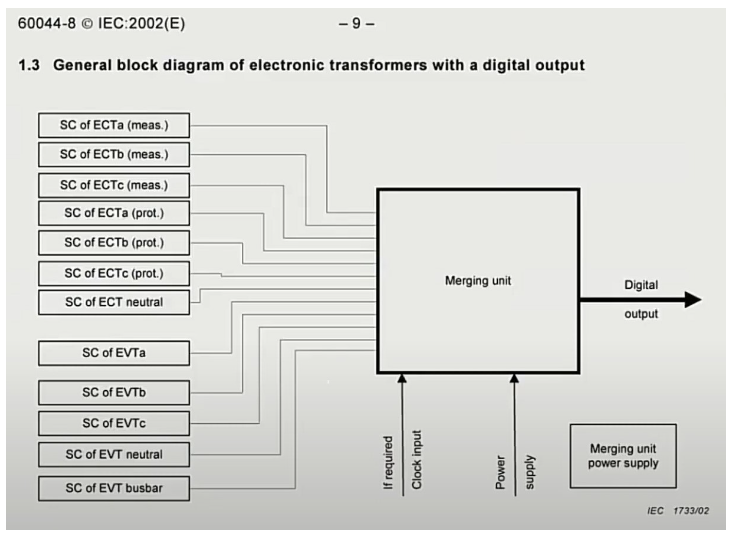
\includegraphics[width=\textwidth, keepaspectratio]{ch2/assets/Idea_of_Merging_Unit.png}
	\caption{Concept of the Merging Unit.}
	\label{fig:Merging-Unit}
\end{figure}
\FloatBarrier

\subsection{IEC~61850-9-1/2003}

This marks the beginning of the protocol known today. However, it initially leaned towards a point-to-point communication model, resembling its predecessor IEC 60044. This approach lacked considerations for network applications, crucial for the interoperability that the protocol now provides. The concept of the Process Bus network, prevalent today, was not present during this period, causing delays in releasing the next version (~\cite{History_Sample_Value}).

\subsection{IEC~61850-9-2(Ed1)/2004}

At this stage, the abstraction of the IEC 61850 standard is being carefully applied once more. Initially introduced in the IEC 61850-7-2 standard, this service specification has since developed into a well-defined standard within IEC 61850-9-2, where it is clearly outlined within the context of Ethernet communication.

The data structure is characterized by its generic definition, and the communication process operates entirely independently. This implies that, in the future, we could seamlessly transition to another standard beyond Ethernet, tailored to the system's evolving needs. This flexibility is a testament to the power that abstraction brings. However, it's important to note that, thus far, the Ethernet protocol has been utilized and has consistently met the expected performance requirements.

In this revised standard, the noteworthy inclusion is the implementation of the process bus for Sampled Values, signaling a departure from the initial point-to-point communication approach. Here, to propagate Ethernet packets across the network, it leverages the existing multicast definition of the Ethernet protocol.

A widely embraced guideline employed by manufacturers in the development of Sampled Values is the UCA Implementation Guideline for IEC 61850-9-2.. It's crucial to recognize that this is a guideline, not a standard(~\cite{History_Sample_Value}).

\subsection{IEC 61850-9-2 Ed2/2011}

In this new edition, there were not many changes, mainly due to the fact that the energy industry was not significantly progressing in the adoption of this technology, even with lighter versions like IEC~61850-9-2-LE. The reasons for this lack of progress are attributed to the skeptical nature of many protection engineers. They tend to be more conservative when it comes to supplying electrical power, sometimes justified by negative experiences in the field(~\cite{History_Sample_Value}).

There were also some technical issues with SVs due to time synchronization. At that time, the most used protocol was SNTP, which allowed only millisecond precision. For SVs, higher precision in samples was needed. Additionally, there was immaturity in redundancy solutions in the network. Consequently, these two significant problems were only resolved later with the implementation of the following technologies:

\begin{itemize}
	\item Time Synchronization - Precision Time Protocol (PTP): This protocol enables time synchronization via Ethernet with a timing error of less than 1 microsecond. Synchronization could now be achieved through the Ethernet network connection, eliminating the need for a separate network for time synchronization of merging units in the field.
	\item Redundancy - Parallel Redundancy Protocol (PRP): PRP operates with effectively two duplicated networks, resembling the approach adopted by service providers in the transmission of electrical energy networks. These providers often maintain redundant protection/control systems. The loss of service in one of these networks does not compromise functionality, as the parallel network continues to perform its communication functions without affecting the protection/control systems.
	\item High Availability Continuous Redundancy (HSR): HSR provides redundancy through a ring architecture. This is essentially the same ring architecture, where communication service continuity is maintained through the open ring, in case of service loss in any part of the closed ring. In both cases, specific hardware (and software) requirements must be met to consider the implementation of the solution. This is a fundamental element in the design of the Digital Substation.
\end{itemize}

For time synchronization, the adopted solution was the Precision Time Protocol (PTP). With a resolution below 1 microsecond, this was sufficient for SVs to be synchronized, making it possible to reconstruct the digital waveform into analog again and check for faults or network issues by IEDs. In terms of redundancy, two solutions were implemented: PRP and HSR, with PRP being the more widely used due to lower associated implementation costs and the assurance of redundancy(~\cite{History_Sample_Value}).

\subsection{IEC 61869-9/2016}

The IEC 61869-9 standard is familiar to everyone using instrument transformers for other applications in the industry. This standard provided recommendations for measuring instruments, ranging from light versions to more demanding ones. The Figure~\ref{fig:SV-Tables} below summarizes this information.~\footnote{\url{https://www.linkedin.com/pulse/history-iec-61850-sampled-values-tibor-congo/}}

\begin{figure}[tbh]
	\centering
	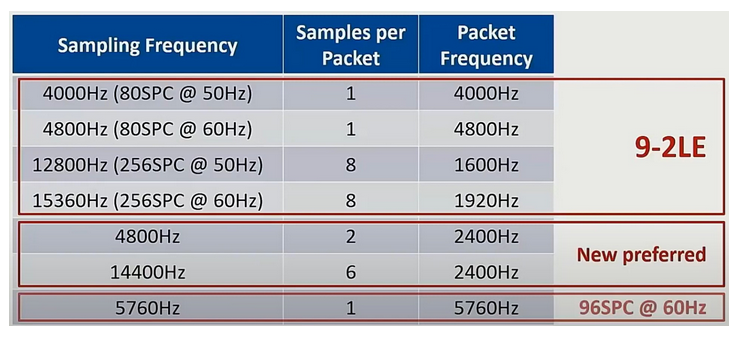
\includegraphics[width=\textwidth, keepaspectratio]{ch2/assets/table_SVs_Frequency.png}
	\caption{Frequency regarding Sampled Values.}
	\label{fig:SV-Tables}
\end{figure}
\FloatBarrier

The information derived from the table indicates that protection functions use a sampling rate of 4800Hz at 60Hz and 4000Hz at 50Hz according to the IEC~61850-9-2-LE version. When we talk about preferred streams, the sampling rates remain the same regardless of their use, such as protection, measurement, or power quality. This balance is achieved by adjusting the necessary samples per Application Specific Data Unit (ASDUs) per packet.

The IEC61869-9 standard mentions the use of configurable datasets. The IEC 61850-9-2-LE version simplified this by publishing 4 currents + 4 voltages for all datasets. While this approach was efficient, it lacked flexibility. Therefore, IEC61869-9 introduces flexibility in this regard, optimizing the implementation. However, this increased flexibility also brings greater complexity to data processing(~\cite{History_Sample_Value}).

\subsection{IEC~61850-9-2 Ed2.1/2020}

In this latest update, there was a small reinforcement of what was mentioned in the previous version. Here, a new field called SynchSrcID was introduced, which is used to specify the synchronization source of the merging unit. This new feature is one of the optional fields. In the IEC~61850-9-2-LE version, there was only one field, but breaking free from the limitations of this version, now there are more fields to configure. Again, a note on what was mentioned above, it is essential to analyze configuration issues and implementation costs, as it will be more complex(~\cite{History_Sample_Value}).\newline


The evolution from IEC 60044-8 to IEC 61850-9-2 ED2.1 marks the shift from analog to digital in substation communication. Starting with the digitization of transformer outputs, it progressed through increasingly sophisticated standards (IEC 61850-9-1, 9-2 ED1, and 9-2 LE), refining the transmission of sampled values over Ethernet. The development culminated in IEC 61869-9 and IEC 61850-9-2 ED2.1, which ensure interoperability and advanced digital communication in modern substations, in Figure~\ref{fig:Evolution of IEC 61850-9-2} ~\footnote{\url{https://www.linkedin.com/pulse/history-iec-61850-sampled-values-tibor-congo/}} has showned the progress through years.

\begin{figure}[tbh]
	\centering
	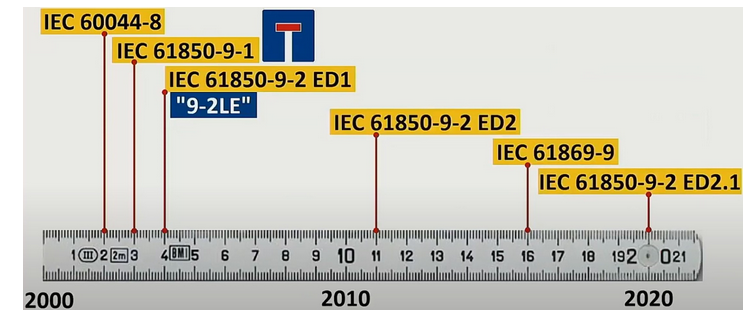
\includegraphics[width=\textwidth, keepaspectratio]{ch2/assets/evolucao_SV_protocol.png}
	\caption{Evolution of IEC 61850-9-2}
	\label{fig:Evolution of IEC 61850-9-2}
\end{figure}


\FloatBarrier
